\documentclass[12pt,a4paper]{article}
%-- coding: UTF-8 --
\usepackage[UTF8]{ctex}
\usepackage[utf8]{inputenc}
\usepackage{geometry}
\usepackage{graphicx} % 引入图片
\usepackage{enumitem} % 取消列表默认间距
\geometry{left=3.18cm,right=3.18cm,top=2.54cm,bottom=2.54cm}
\usepackage{hyperref}
\hypersetup{hidelinks,
	colorlinks=true,
	allcolors=black,
	pdfstartview=Fit,
	breaklinks=true}
\usepackage{listings}
\usepackage{xcolor}
\usepackage{fontspec}
\usepackage{booktabs} % 三线表
\usepackage{float}

\usepackage{tikz}
\usepackage{amsmath}
\usepackage{colortbl}
\newcommand\y{\cellcolor{clight2}}
\definecolor{clight2}{RGB}{212, 237, 244}%
\newcommand\tikznode[3][]%
   {\tikz[remember picture,baseline=(#2.base)]
      \node[minimum size=0pt,inner sep=0pt,#1](#2){#3};%
   }
\tikzset{>=stealth}
\renewcommand\vec[1]{\mathbf{#1}}

% 嵌入代码风格
\lstset{
	language    = c++,
	breaklines  = true,
	captionpos  = b,
	tabsize     = 4,
	columns     = fullflexible,
	commentstyle = \color[RGB]{0,128,0},
	keywordstyle = \color[RGB]{0,0,255},
	basicstyle   = \small\ttfamily,
	stringstyle  = \color[RGB]{148,0,209}\ttfamily,
	rulesepcolor = \color{red!20!green!20!blue!20},
	showstringspaces = false,
}


%伪代码
\usepackage{multirow}
\usepackage{algorithm}
\usepackage[noend]{algpseudocode}
\usepackage{amsmath}

\title{实验六 \hspace{0.5cm} 图的最短路径与最小生成树算法}
\author{}
\date{December, 2023}

\begin{document}
\maketitle

\section{前言}
1736年29岁的欧拉向圣彼得堡科学院递交了《哥尼斯堡的七座桥》的论文,在解答问题的同时,开创了数学的一个新的分支——图论与几何拓扑,也由此展开了数学史上的新历程。七桥问题提出后,很多人对此很感兴趣,纷纷进行试验,但在相当长的时间里,始终未能解决。欧拉通过对七桥问题的研究,不仅圆满地回答了哥尼斯堡居民提出的问题,而且得到并证明了更为广泛的有关一笔画的三条结论,人们通常称之为“欧拉定理”。

图模拟一组连接,由节点和边组成。一个图就是一些顶点的集合,这些顶点通过一系列边结对(连接)。顶点用圆圈表示,边就是这些圆圈之间的连线,顶点之间通过边连接。图计算是研究客观世界当中的任何事物和事物之间的关系,对其进行完整的刻划、计算和分析的一门技术。图计算技术主要是由点和边来组成的。举例来说,点可以是坐在演播室里的三个人,这三个人就是三个点,所谓的边就是这三个人之间的关系。比如说,同事关系、亲戚关系、夫妻关系等,而且两个人之间的关系不仅限于一种描述,还可能有一些其他的关系,比如说项目合作关系、投资关系等。原则上两点之间的关系没有上限,可以有很多的各种关系。点越多,当然各点相互之间可能的关系也就越错综复杂。

图 $G$ 由节点 $V$(vertice)与边 $E$(edge)构成,我们一般表示为 $G(V,E)$。图数据的典型例子比如网页链接关系、社交网络、商品推荐等。比如微信的社交网络,是由节点(个人、公众号)和边(关注、点赞)构成的图;淘宝的交易网络,是由节点(个人、商品)和边(购买、收藏)构成的图。如此一来,抽象出来的图数据构成了研究和商用的基础,可以以此探究出“世界上任意两个人之间的人脉距离”,“关键意见领袖”等。将这些应用到商业领域,其底层的运算往往是图相关的算法,这便是图计算。

在金融行业中,图计算以及认知技术重点应用的业务领域包括:金融风险的管控、客户的营销拓展,内部的审计监管、以及投资理财等方面。再如国内商业银行都面临的信贷风险问题:受国内经济下行的影响,企业客户贷款的不良率攀升。为了提高银行对企业不良风险传导的预测能力,利用图计算和图认知技术,完整刻画企业客户之间、企业与自然人之间的社会关系、经济往来关系,构建全方位的风险关联网络,实现风险要素的动态性和完整性呈现。图计算模型在大数据公司,尤其是 IT 公司是非常流行的一大模型,它是很多实际问题最直接的解决方法。近几年,随着数据的多样化,数据量的大幅度提升和算力的突破性进展,超大规模图计算在大数据公司发挥着越来越重要的作用,尤其是以深度学习和图计算结合的大规模图表征为代表的系列算法。图计算的发展和应用有井喷之势,各大公司也相应推出图计算平台,例如 Google Pregel、Facebook Giraph、腾讯星图、华为图引擎服务 GES 等。



\section{实验项目结构}

\begin{itemize}[noitemsep]
    \item[$-$] 1\_shortest\_path \textit{题目一 \hspace{0.1cm} 最短路径问题}
    \begin{itemize}[noitemsep]
        \item[$-$] include
        \begin{itemize}[noitemsep]
            \item[$\bullet$] util.hpp \textit{常用函数头文件}
            \item[$\bullet$] Solution.hpp \textit{待完成}
        \end{itemize}
        \item[$-$] data
        \item[$\bullet$] main.cpp \textit{主程序代码}
    \end{itemize}
    \item[$-$] 2\_minimun\_spanning\_tree \textit{题目二 \hspace{0.1cm} 最小生成树问题}
    \begin{itemize}[noitemsep]
        \item[$-$] 略
    \end{itemize}
    \item[$-$] 3\_minimun\_spanning\_tree\_plus \textit{题目三 \hspace{0.1cm} 最小生成树问题 Plus(拓展题)}
    \begin{itemize}[noitemsep]
        \item[$-$] 略
    \end{itemize}
    \item[$-$] 4\_building\_roads \textit{题目四 \hspace{0.1cm} 道路建设(拓展题)}
    \begin{itemize}[noitemsep]
        \item[$-$] 略
    \end{itemize}
\end{itemize}

\textcolor{red}{请注意,每次修改完代码之后,需要重新编译运行 main.cpp,如果直接执行上次编译好的 main.exe 或 main,新的修改将不会生效。在本地测试通过后请将代码提交到 OJ 上。}

\section{实验内容}

\subsection{最短路径问题}
给定 $n$ 个点( $1\sim n$ 表示),$m$ 条边构成的无向连通图(任意两点互相可达)。第 $i$ 条边 $edges[i] = \{x, y, z\}$ 表示 $x$ 与 $y$ 之间有一条长度为 $z$ 的无向边。请你求出从 $1$ 号点到 $n$ 号点的最短路距离。


\begin{lstlisting}
    class Solution {
    public:
        long long shortest_path(int n, vector<vector<int>>& edges) {
            // 请在这里完成你的代码
        }
    };
\end{lstlisting}

\textbf{注:请使用 Dijkstra算法 求解。}

数据范围:100\% 的数据满足:$1\le n \le 10^3, 1 \le m \le 10^5, 1 \le z \le 10^9$



\subsection{最小生成树问题}
给定 $n$ 个点( $1\sim n$ 表示),$m$ 条边构成的无向连通图(任意两点互相可达)。第 $i$ 条边 $edges[i] = \{x, y, z\}$ 表示 $x$ 与 $y$ 之间有一条长度为 $z$ 的无向边。请你求出最小生成树的边权和。

\begin{lstlisting}
    class Solution {
    public:
        long long minimum_spanning_tree(int n, vector<vector<int>>& edges) {
            // 请在这里完成你的代码
        }
    };
\end{lstlisting}

\textbf{注:请使用 Prim算法 求解。}

数据范围:100\% 的数据满足:$1\le n \le 10^3, 1 \le m \le 10^5, 1 \le z \le 10^9$




\section{实验思考}

\begin{enumerate}
    \item 你所使用的 Dijkstra 算法的时间复杂度是多少?还有可能的优化空间吗?
    \item 如果要输出具体的最短路径(包括路径上的点和路径上的边),你的代码应该如何修改?(仅说明需要哪些新的数组以及如何使用即可,不需要重写代码)
    \item 你所使用的 Prim 算法的时间复杂度是多少?还有可能的优化空间吗?
    \item 如果要输出具体的最小生成树,你的代码应该如何修改?(仅说明需要哪些新的数组以及如何使用即可,不需要重写代码)
    
\end{enumerate}

\section{拓展实验}

\subsection{题目 I 最小生成树 Plus}

给定 $n$ 个点( $1\sim n$ 表示),$m$ 条边构成的无向连通图(任意两点互相可达)。第 $i$ 条边 $edges[i] = \{x, y, z\}$ 表示 $x$ 与 $y$ 之间有一条长度为 $z$ 的无向边。请你求出最小生成树的边权和。

\begin{lstlisting}
    class Solution {
    public:
        long long minimum_spanning_tree(int n, vector<vector<int>> edges) {
            // 请在这里完成你的代码
        }
    };
\end{lstlisting}

数据范围:100\% 的数据满足:$1\le n \le 10^5, 1 \le m \le min(\frac{n(n-1)}{2}, 10^6), 1 \le z \le 10^9$

\textbf{注:请使用 Kruskal算法 求解。}如果你不清楚如何对边按照边权进行排序,请参考 lab5 实验指导书的附录部分

\subsection{题目 II 道路建设}

市长 Bob 所管理的城市由 $n$ 个社区(编号 $0\sim n-1$)组成,由于疫情封控需要保证每个社区的物资供应。在第 $i$ 个社区建立物资供应站需要花费 $w_i$ 元。

为了节省建立物资供应站的经费开销,Bob 提供了 $m$ 个道路建设方案,第 $i$ 个方案 $\{x, y, z\}$ 表示在 $x$ 社区向 $y$ 社区修一条路需要花费 $z$ 元。只要每个社区能够收到物资供应,就符合要求。Bob 保证这 $m$ 条道路能够使 $n$ 个社区连通,请你帮忙求出最经济的建设方案。

提示:只要社区建立了物资供应站,或者与某个建立了物资供应站的社区相连通,那么该社区就可以收到物资供应。
\begin{lstlisting}
    class Solution {
    public:
        long long build_roads(int n, vector<int>& w, vector<vector<int>>& edges){
            // 请在这里完成你的代码
        }
    };
\end{lstlisting}
\begin{figure}[h]
    \centering
    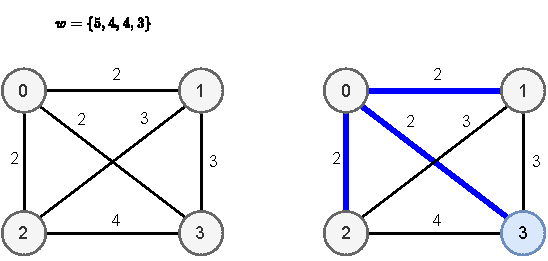
\includegraphics[width=12cm]{img/lab6/build_roads.pdf}
    \caption{道路建设例子}
    \label{fig:build_roads}
\end{figure}

如图 \ref{fig:build_roads} 所示,左侧图表示有 0 - 3 共 4 个社区,建设物资供应站的费用依次为 5,4,4,3 元,另外还有 6 条边使得这 4 个社区连通。右侧图是最省钱的方案,我们选择 3 号社区建立物资供应站,然后选择 3 条边权为 2 的边。


数据范围:100\% 的数据满足:$1\le n \le 10^5, 1 \le m \le min(\frac{n(n-1)}{2}, 10^6), 1 \le w[i], z \le 10^9$

\section{附录}

\subsection{图的存储}

图的表示方法有很多种,按照底层数据结构可以分为顺序表存储和链式表存储。图分为点集和边集两部分,我们一般仅考虑边的存储方式。

设 $n$ 为图的点数,$m$ 为图的边数。

\subsubsection{边集存储}

边集存储是最简单的存储方式,它是一个数组,将所有边依次存放起来。
\begin{lstlisting}
    const int M = 1000000;
    struct Edge{
        int x, y;
    }e[M];
\end{lstlisting}

更为一般的,我们也可以用一个长度为 2 的 vector 数组来表示一条边(有向或无向),然后用一个 vector 数组将这些边存储起来。
\begin{lstlisting}
    vector<vector<int>> edegs = {{1, 2}, {2, 3}, {1, 3}};
    for(auto &edge : edges) {
        cout << edge[0] << ' ' << edge[1] << endl;
    }
\end{lstlisting}

二维数组 edges 包含了 3 条边,每条边 edge 用一个一维数组存放,edge[0] 和 edge[1] 分别是边的两个端点。如果要表示带权图,那么 edge 将是一个长度为 3 的数组,edge[2] 表示对应边的权值。

不论是自定义结构体还是直接使用 vector,他们的空间复杂度都是 $O(m)$,但是想要找到某个点连接的所有边是不容易的,复杂度为 $O(m)$。这种存图方式不经常使用,但不可否认它是所有存图方式中,最简单也最直接的一种方式。

\subsubsection{邻接矩阵}

领接矩阵可以用一个大小为 $n\times n$ 的二维数组表示。在不带权的图中,矩阵元素仅由 0 和 1 构成即可表示整张图。而在带权图中,我们可以提前预设一个值(例如无穷大 inf)表示边不存在,而其他值表示对应边的权值。

\begin{lstlisting}
    const int N = 1000;
    int adj[N][N];
    
    memset(adj, 0x3f, sizeof adj); 
    int n, m;
    cin >> n >> m;
    for(int i = 1; i <= m; i++) {
        int u, v, w;
        cin >> u >> v >> w;
        adj[u][v] = adj[v][u] = w; // 无向带权图
    }
\end{lstlisting}

上述代码展示了如何使用领接矩阵存无向带权图。其中的 memset 函数是指将 adj 数组的每个字节都赋值为 0x3f,因为 int 是 4 个字节,所以最终 adj 中的每个元素都等于 0x3f3f3f3f,这是一个十六进制数字,在十进制下为 1061109567,可以用来表示 inf。

邻接矩阵的优势在于可以 $O(1)$ 的访问一条边,劣势在于空间复杂度为 $O(n^2)$,通常只能保存点数为 $10^3$ 规模的图。(因为$10^6$ 个 int 内存占用接近 4MB)

\subsubsection{邻接表}

通常,邻接表是指 adj[u] 存放了 u 指向的所有点,用链表实现。但其实更简单的方法是一个使用 vector。

\begin{lstlisting}
    int n, m;
    cin >> n >> m;
    vector<vector<pair<int, int>>> adj(n); //创建 n 个二维数组,下标范围 0 ~ n-1
    for(int i = 1; i <= m; i++) {
        int u, v, w;
        cin >> u >> v >> w;
        adj[u].push_back(make_pair(v, w));  // 方式 1
        adj[v].push_back({u, w});           // 方式 2
    }
\end{lstlisting}

上述展示了如何使用 vector 二维数组来表示无向带权图。我们使用 push\_back() 动态的向 vector 中添加元素,这保证了总体空间是 $O(m)$ 的。另外,为了存放边权,我们使用 pair<int,int> 二元组,你可以通过下面的方式访问 u 连接的所有边:

\begin{lstlisting}
    for(int i = 0; i < adj[u].size(); i++) {
        cout << u << ' ' << adj[u][i].first << ' ' << adj[u][i].second << endl;
    }
\end{lstlisting}

如你所见,你可以通过 first 和 second 来分别访问 pair<int,int> 中的第一个和第二个元素。

\subsection{最短路径问题}

最短路径问题有很多,我们这里仅讨论单源最短路径问题,并且仅局限于 Dijkstra 算法来解决该问题。

单源最短路径:给定一个有向图 $G=(V, E)$,节点以 [1,n] 之间的连续整数编号,$(u,v,w)$ 描述一条从 $u$ 出发,到达 $v$,边权为 $w$ 的有向边。设 $1$ 号点为起点,求长度为 $n$ 的数组 $dist$,其中 $dist[i]$ 表示从起点 $1$ 到节点 $i$ 的最短路径长度。

$Dijkstra$ 算法:
\begin{enumerate}[itemsep=0 pt]
    \item 初始化 $dist[1] = 0$,其余节点 $dist$ 值为正无穷大。
    \item 找出一个未标记的、$dist[x]$ 最小的节点 $x$,然后标记 $x$。(对应于 EXTRACT-MIN 操作)
    \item 扫描 $x$ 的出边 $(x, y, z)$,若 $dist[y] > dist[x] + z$,则更新 $dist[y] = dist[x] + z$。(对应于 RELAX 操作)
    \item 重复上述三个步骤,直到所有的节点都被标记。
\end{enumerate}

$Dijkstra$ 算法基于贪心思想,它只适用于所有边的权值都是非负数的图。

在第 2 步选出的 $x$,其 $dist[x]$ 已经是起点到 $x$ 的最短距离。我们不断选择全局最小值进行标记和扩展,最终可得到起点到每个节点的最短路长度。

\subsection{最小生成树问题}

最小生成树问题主要有两个方法:$Prim$ 算法和 $Kruskal$ 算法。这两个算法都基于一个推论:

给定一张无向图 $G=(V,E),n = |V|, m = |E|$。从 $E$ 中选出 $k < n-1$ 条边构成 $G$ 的一个生成森林。若再从剩余的 $m-k$ 条边中选 $n-1-k$ 条边添加到生成森林中,使其称为 $G$ 的最小生成树,\textbf{则最小生成树一定包含这 $m-k$ 条边中权值最小的边,且该边的两个端点不在同一颗树中}。

\subsubsection{Prim 算法}

任意时刻,设已经确定属于最小生成树的节点集合 $T$(起初只有 1 号点),剩余节点集合为 $S$,$Prim$ 算法每次需要找到一条边 $i$,它的边权 $z_i$ 满足:
$$z_i = \min_{(x,y,z) \in E, x\in S, y\in T}z$$

即该边两个端点分别属于集合 $S$ 和 $T$,并且权值最小。然后 $Prim$ 算法将 $x$ 点从 $S$ 中删除,加入到 $T$ 集合,并把 $z$ 累加到答案中。

在过程中,我们维护一个数组 $d$:

\begin{itemize}[noitemsep]
    \item 若 $x\in S$,则 $d[x]$ 表示 $x$ 与集合 $T$ 中的节点之间最小的边权。
    \item 若 $x \in T$,则 $d[x]$ 表示 $x$ 被加入 $T$ 时选出的最小边的边权。
\end{itemize}

然后再用一个数组 $v$ 标记节点是否属于 $T$ (即是否被选过),每次从未标记的点中选一个 $d$ 值最小的,把它标记(新加入 $T$),同时扫描所有出边,更新 $S$ 中其他点的 $d$ 值。

最后生成树的权值之和就是 $\sum_{x=1}^n d[x]$。

\subsubsection{Kruskal 算法}

Kruskal 算法是一种用来查找最小生成树的算法,由Joseph Kruskal在1956年发表。用来解决同样问题的还有Prim算法和Boruvka算法等。三种算法都是贪心算法的应用。和Boruvka算法不同的地方是,Kruskal算法在图中存在相同权值的边时也有效。

该算法的步骤如下:

\begin{enumerate}[itemsep=2pt,topsep=0pt,parsep=0pt]
    \item 新建图 $G$, $G$中拥有原图中相同的节点,但没有边
    \item 将原图中所有的边按权值从小到大排序
    \item 从权值最小的边开始,如果这条边连接的两个节点于图$G$中不在同一个连通分量中,则添加这条边到图$G$中
    \item 重复3,直至图$G$中所有的节点都在同一个连通分量中
\end{enumerate}

\begin{figure}
    \centering
    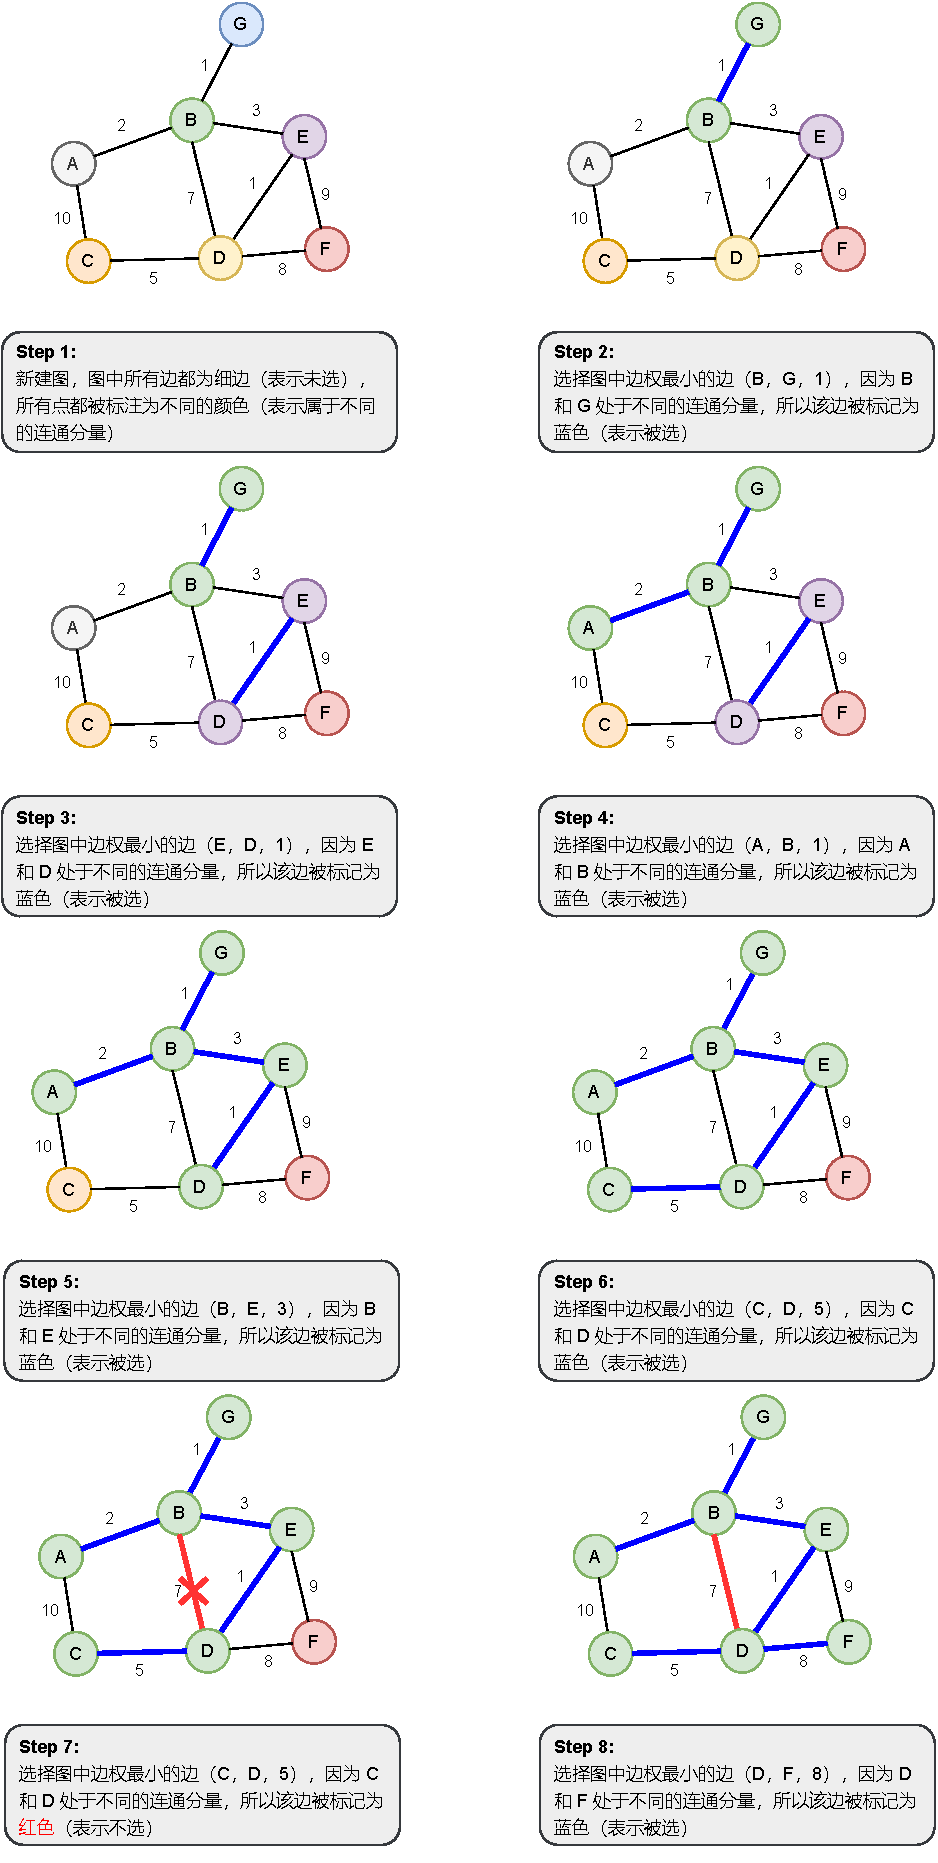
\includegraphics[width=12cm]{img/lab6/kruskal.pdf}
    \caption{kruskal 求解过程}
    \label{fig:kruskal}
\end{figure}


图 \ref{fig:kruskal} 展示了 Kruskal 的求解过程。Kruskal 的时间复杂度为 $O(m\log m)$,其中对边进行排序的复杂度为 $O(m\log m)$。依次遍历每条边,判断两端点是否属于同一个连通分量的复杂度可以非常小,使用并查集实现。

\subsection{并查集}
\begin{figure}[h]
    \centering
    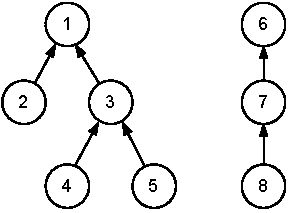
\includegraphics{img/lab6/并查集.pdf}
    \caption{并查集结构}
    \label{fig:uf}
\end{figure}

并查集是一种树形的数据结构,顾名思义,它用于处理一些不交集的\textbf{合并}及\textbf{查询}问题。 它支持两种操作:

\begin{enumerate}[itemsep=2pt,topsep=0pt,parsep=0pt]
    \item 查找(Find):确定某个元素处于哪个子集;
    \item 合并(Union):将两个子集合并成一个集合。
\end{enumerate}

在上图中,分别有两个集合 $\{1, 2, 3, 4, 5\}$ 和 $\{6, 7, 8\}$,如果用 $f[x]$ 表示$x$在树中的父亲,那么就有 $f[2] = 1, f[4] = 3, f[8] = 7$。特殊的,令树根的父亲是树根自己,即 $f[1] = 1, f[6] = 6$。

在判断某两个元素是否属于同一集合时,首先分别找到其所在集合的根节点,如果根节点是同一个,那么表示这两个元素属于同一集合,否则表示这两个元素属于不同的集合。例如,在判断 4 和 5 是否属于同一集合时,分别通过递归找到其根节点都为 1,所以它们属于同一集合。再例如,判断 3 和 7 是否属于同一集合时,分别找到它们的根节点是 1 和 6,1 不等于 6,所以它们属于不同的集合。

\subsubsection{初始化}

一般初始化时,我们让所有点都指向自己,表示每个点都是一个独立的集合。
\begin{lstlisting}
    vector<int> f(n);
    for(int i = 0; i < n; i++) {
        f[i] = i;
    }
\end{lstlisting}
\subsubsection{查找}

\begin{figure}[h]
    \centering
    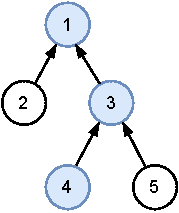
\includegraphics{img/lab6/并查集_get.pdf}
    \caption{在并查集中查找 4 的根结点}
    \label{fig:uf_get}
\end{figure}

在并查集中查找 4 的根节点的过程:

\begin{enumerate}[itemsep=2pt,topsep=0pt,parsep=0pt]
    \item $f[4] = 3$,继续查找 3 的根节点
    \item $f[3] = 1$,继续查找 1 的根节点
    \item $f[1] = 1$,1 就是根节点,返回结果 1
\end{enumerate}

代码如下:
\begin{lstlisting}
    int find(int x) {
        return x == f[x] ? x : find(f[x]);
    }
\end{lstlisting}

\subsubsection{路径压缩}

由于并查集仅支持合并和查询,在整个过程中集合不会被拆解,树只会在原来的基础上增加。因此,为了加快查找速度,我们会在每次查询结束后对路径进行压缩。

\begin{figure}[h]
    \centering
    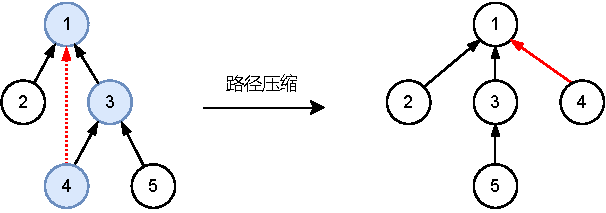
\includegraphics{img/lab6/并查集_路径压缩.drawio.pdf}
    \caption{并查集的路径压缩}
    \label{fig:uf_cmpression}
\end{figure}

比如,在查询 4 的根节点时,会得到结果 1,紧接着直接修改 $f[4] = 1$。这样做的好处是接下来再次查询时会快很多,省去了多余的查询。从下面的代码中,可以看出我们并不只是对 4 进行修改,而是对从 4 到 1 的路径上的所有节点都进行了修改,正所谓「路径压缩」。

\begin{lstlisting}
    int find(int x) {
        return x == f[x] ? x : f[x] = find(f[x]);
    }
\end{lstlisting}

把在路径上的每个节点都直接连接到根上,这就是路径压缩。

\subsubsection{合并}

\begin{figure}[h]
    \centering
    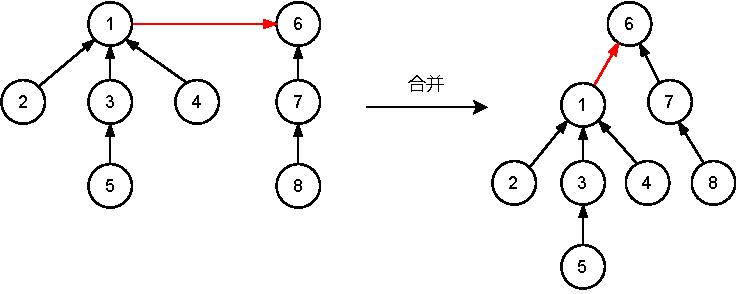
\includegraphics{img/lab6/并查集_union.pdf}
    \caption{并查集的合并}
    \label{fig:uf_union}
\end{figure}

在合并 $x$ 所在集合与 $y$ 所在集合时,我们首先利用 get 函数找到他们对应的根结点 $\textit{root}_x$ 和 $\textit{root}_y$,然后令 $f[\textit{root}_x] = \textit{root}_y$ 即可。

\subsubsection{时间复杂度}

你可以先不严谨的认为,并查集的单个操作都是 $O(1)$ 的。如果想要详细了解相关内容,可以参考:\href{https://zh.wikipedia.org/wiki/并查集}{https://zh.wikipedia.org/wiki/并查集}


\end{document}